\documentclass{jarticle}
\usepackage[dvipdfmx]{graphicx}
\usepackage{bm}
\usepackage{amsmath,amssymb}
\begin{document}
\begin{flushleft}
{\large
 逆格子ベクトルを求める}
\begin{enumerate}
\item はじめに
     \\結晶の性質を調べる際に使われる数学的概念として逆格子ベクトルがある。
     \\逆格子ベクトルは実格子ベクトル$\vec{a_1}$,$\vec{a_2}$,$\vec{a_3}$を用いて
 \begin{equation}
   \vec{b_1}=\frac{2\pi\vec{a_2}×\vec{a_3}}{V}
 \end{equation}
 \begin{equation}
   \vec{b_2}=\frac{2\pi\vec{a_3}×\vec{a_1}}{V}
 \end{equation}
 \begin{equation}
   \vec{b_3}=\frac{2\pi\vec{a_1}×\vec{a_2}}{V}
 \end{equation}
 と定義される。ここでVは$\vec{a_1}$,$\vec{a_2}$,$\vec{a_3}$のベクトルが作る体積である。
 \begin{center}
 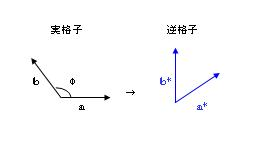
\includegraphics[width=6cm]{lattice.jpg}
 \end{center}
\item 目的
\\三組の実格子ベクトルが指定されたときにその結晶の逆格子ベクトルを求めること。
\item 方法
\\一般のベクトル$\vec{a_1}$,$\vec{a_2}$,$\vec{a_3}$に対して逆格子の定義からfortran90を用いて計算をする。
後から任意の成分を入力出来るようにした。
\item 結果
\\例えば
\begin{equation}
  \vec{a_1}=(1,0,0),\vec{a_1}=(0,1,0),\vec{a_3}=(0,0,1)
\end{equation}
に対して

  \begin{equation}
    \vec{b_1}=(6.2831854820251465,0,0)=(2\pi,0,0)
  \end{equation}
  \begin{equation}
    \vec{b_2}=(0,6.2831854820251465,0)=(0,2\pi,0)
  \end{equation}
  \begin{equation}
    \vec{b_3}=(0,0,6.2831854820251465)=(0,0,2\pi)
  \end{equation}
となった。
\end{enumerate}




\end{flushleft}
\end{document}
